\pgfplotsset{width=0.8\linewidth,height=9em,compat=1.18}
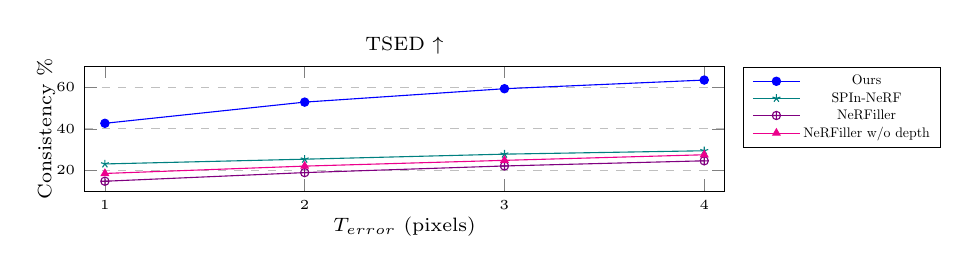
\begin{tikzpicture}
    \begin{axis}[
        title style={align=center, font=\scriptsize, yshift=-.5em},
        title={TSED $\uparrow$},
        xlabel={$T_\text{error}$ (pixels)},
        ylabel={Consistency \%},
        xmin=0.9, xmax=4.1,
        ymin=10, ymax=70,
        xtick={1,2,3,4},
        ytick={20,40,60},
        legend pos=outer north east,
        legend style={nodes={scale=0.5, transform shape}},%
        label style={font=\scriptsize},
        tick label style={font=\tiny},
        ymajorgrids=true,
        grid style=dashed,
        xlabel style={yshift=1ex},
        ylabel style={yshift=-1.5ex},
        mark size=1.5pt,x
    ]
        \addplot[color=blue,mark=*,] coordinates {
        (1.0,42.7083)(2.0,52.9167)(3.0,59.3750)(4.0,63.5417)
        };
        \addplot[color=teal,mark=star,] coordinates {
        (1.0,23.1250)(2.0,25.4167)(3.0,27.8472)(4.0,29.4792)
        };
        \addplot[color=violet,mark=oplus,] coordinates {
        (1.0,14.7917)(2.0,18.9583)(3.0,22.1528)(4.0,24.6354)
        };
        \addplot[color=magenta,mark=triangle*,] coordinates {
        (1.0,18.5417)(2.0,22.0833)(3.0,24.8611)(4.0,27.5521)
        };
        \legend{Ours
        ,SPIn-NeRF ,NeRFiller ,NeRFiller w/o depth}
    \end{axis}
\end{tikzpicture}
